\section{Negative Selection Algorithm}

\begin{frame}{Biological immune system}
  \begin{itemize}
  \item {
    The antigen-antibody reaction is an exclusive process.
  }
  \item {
    The primary role of immune system is to distinguish self from non-self.
  }
  \item {
    Immune cells are tolerant to self antigens but activate defense mechanisms when recognize non-self antigens.   
  }
  \item {
    The negative selection of T cells happened in the thymus during maturation.
  }
  \end{itemize}
\end{frame}

\begin{frame}{Biological immune system}
  \begin{figure}[hb]
  \centering
  %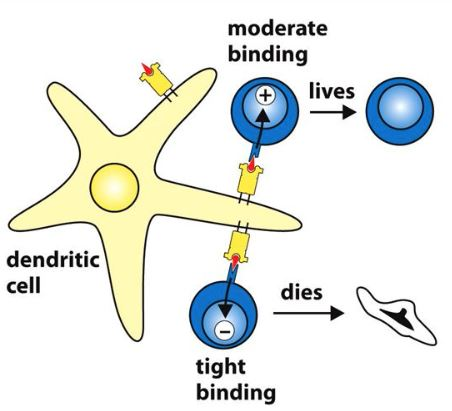
\includegraphics[width=0.6\textwidth]{NSA/figures/NST.JPG}
  \caption{Negative selection of T cells}
  \end{figure}
\end{frame}

\begin{frame}{Biological immune system}
  \begin{figure}[hb]
  \centering
  %\includegraphics[width=0.6\textwidth]{NSA/figures/is.jpg}
  \caption{Antigen-antibody interaction}
  \end{figure}
\end{frame}

% You can reveal the parts of a slide one at a time
% with the \pause command:
\begin{frame}{Defining the NSA}
  \begin{itemize}
  \item<1->{
    Define Self as a normal pattern of activity or stable behavior of a system/process.\\
    -Represent the collection as multiset of S of strings of length \emph{l} over a finite alphabet.
  }
  \item<2-> {   
    Generate a set R of detectors,each of which fails to match any string in S.
  }
  % You can also specify when the content should appear
  % by using <n->:
  
  \end{itemize}
\end{frame}
 
\begin{frame}{Flowchart}
  \begin{figure}[hb]
  \centering
  %\includegraphics[width=0.8\textwidth]{NSA/figures/flowchart1.jpg}
  \caption{Generation of effective detector}
  \end{figure}
\end{frame}

\begin{frame}{Defining the NSA}
  \begin{itemize}
  \item {
    Monitor new observations for changes by continually testing the detectors matching against representatives of S.  If any detector ever matches, a change must have occurred in system behavior.
  }
  \end{itemize}
\end{frame}

\begin{frame}{Flowchart}
  \begin{figure}[hb]
  \centering
  %\includegraphics[width=0.8\textwidth]{NSA/figures/flowchart2.jpg}
  \caption{Self-monitoring}
  \end{figure}
\end{frame}
